\section{Metodologia}
\subsection*{Metodologia}

\begin{frame}{{\sffamily Metodologia de Pesquisa}}
  \begin{block}{}
    Adaptação da classificação por Prodanov e Freitas:
    \begin{itemize}
      % definições por Prodanov and de Freitas
      \item Quanto a Abordagem:
            \SubItem{Qualitativa e quantitativa}%Qualitativa e Quantitativa
      \item Quanto a Natureza: % Pesquisa aplicada, aplicar conhecimentos/resultados gerados em problemas específicos
            \SubItem{Pesquisa aplicada}
      \item Quanto aos Objetivos: % Exploratória, utilizar os dois metodos para coletar informações para construir uma ferramenta melhor.
            \SubItem{Pesquisa exploratória}
      \item Quanto aos Procedimentos: %Documental literatura cinza, Estudo de caso coletar informações diretamente do usuário, Survey, teve teste piloto tbm.
            \SubItem{Pesquisa documental, survey, estudo de caso}
    \end{itemize}
  \end{block}
\end{frame}

\begin{frame}{{\sffamily Desenho de Pesquisa}}
  \begin{figure}
    \centering
    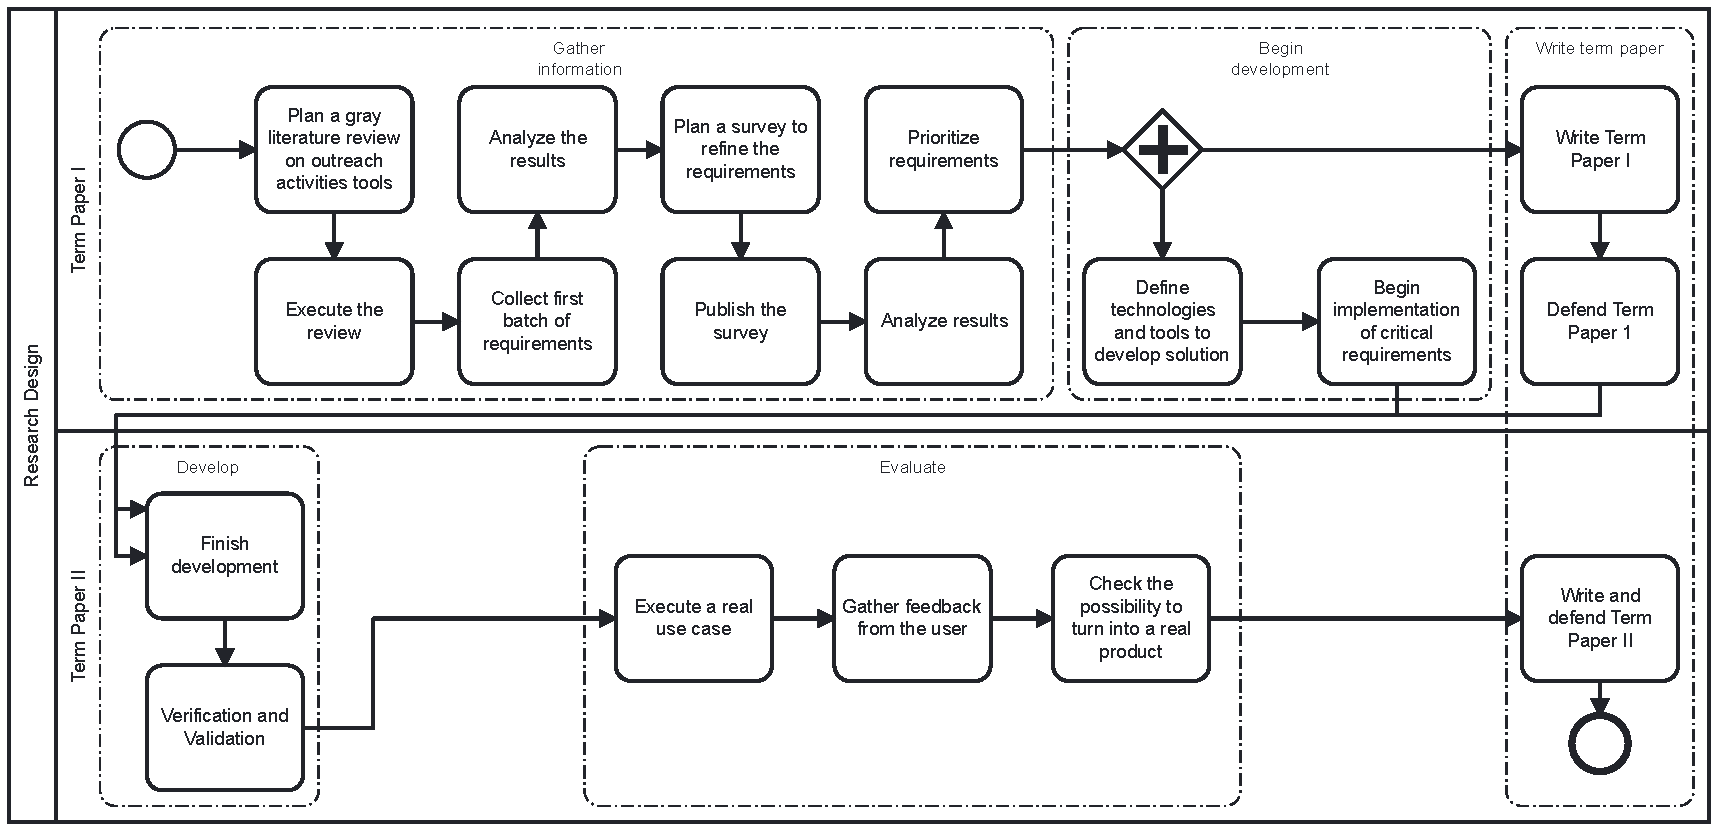
\includegraphics[width=1\textwidth, ]{imagens/2-research design.pdf}
  \end{figure}
\end{frame}

\begin{frame}{{\sffamily Cronograma}}
  \begin{table}[!htb]
  \centering
  \caption{Research Schedule}
  \label{tbl:schedule}
  \scriptsize
  \begin{tabular}{p{4cm}|l|lllll|lll}
    \bottomrule
    \rowcolor[rgb]{0.753,0.753,0.753} \multicolumn{1}{c|}{{\cellcolor[rgb]{0.753,0.753,0.753}}}                                       & \multicolumn{1}{c|}{\textbf{2021/2}} & \multicolumn{5}{c|}{\textbf{2022/1}} & \multicolumn{3}{c|}{\textbf{2022/2}}                                                                                                                                                                                                                                           \\
    \hhline{>{\arrayrulecolor[rgb]{0.753,0.753,0.753}}->{\arrayrulecolor{black}}---------|}
    \rowcolor[rgb]{0.753,0.753,0.753} \multicolumn{1}{c|}{\multirow{-2}{*}{{\cellcolor[rgb]{0.753,0.753,0.753}}\textbf{ Activities}}} & \textbf{Nov - Mar}                   & \multicolumn{1}{c}{\textbf{Apr}}     & \textbf{May}                         & \textbf{Jun}                         & \multicolumn{1}{l}{\textbf{Jul}}     & \textbf{Aug}                         & \textbf{Sep Oct Nov}                 & \textbf{Dec}                         & \multicolumn{1}{c|}{\textbf{Jan}}    \\
    \hline
    \rowcolor[rgb]{0.914,0.914,0.914} Plan and execute systematic review in the grey literature                                       & {\cellcolor[rgb]{0.753,0.753,0.753}} &                                      &                                      &                                      &                                      &                                      &                                      &                                      &                                      \\
    Plan and execute survey with target users                                                                                         &                                      & {\cellcolor[rgb]{0.753,0.753,0.753}} &                                      &                                      &                                      &                                      &                                      &                                      &                                      \\
    \rowcolor[rgb]{0.914,0.914,0.914} Analyze results from previous steps and map requirements                                        &                                      & {\cellcolor[rgb]{0.753,0.753,0.753}} & {\cellcolor[rgb]{0.753,0.753,0.753}} &                                      &                                      &                                      &                                      &                                      &                                      \\
    Plan and start tool development                                                                                                   &                                      &                                      & {\cellcolor[rgb]{0.753,0.753,0.753}} & {\cellcolor[rgb]{0.753,0.753,0.753}} &                                      &                                      &                                      &                                      &                                      \\
    \rowcolor[rgb]{0.914,0.914,0.914} Write Term Paper I                                                                              &                                      &                                      &                                      & {\cellcolor[rgb]{0.753,0.753,0.753}} & {\cellcolor[rgb]{0.753,0.753,0.753}} & {\cellcolor[rgb]{0.753,0.753,0.753}} &                                      &                                      &                                      \\
    Defend Term Paper I                                                                                                               &                                      &                                      &                                      &                                      &                                      & {\cellcolor[rgb]{0.753,0.753,0.753}} &                                      &                                      &                                      \\
    \rowcolor[rgb]{0.914,0.914,0.914} Continue the development of the tool                                                            &                                      &                                      &                                      &                                      &                                      & {\cellcolor[rgb]{0.753,0.753,0.753}} & {\cellcolor[rgb]{0.753,0.753,0.753}} & {\cellcolor[rgb]{0.753,0.753,0.753}} &                                      \\
    Execute a real use case on the tool                                                                                               &                                      &                                      &                                      &                                      &                                      &                                      &                                      & {\cellcolor[rgb]{0.753,0.753,0.753}} &                                      \\
    \rowcolor[rgb]{0.914,0.914,0.914} Write Term Paper II                                                                             &                                      &                                      &                                      &                                      &                                      &                                      &                                      & {\cellcolor[rgb]{0.753,0.753,0.753}} & {\cellcolor[rgb]{0.753,0.753,0.753}} \\
    Defend Term Paper II                                                                                                              &                                      &                                      &                                      &                                      &                                      &                                      &                                      &                                      & {\cellcolor[rgb]{0.753,0.753,0.753}} \\
    \toprule
  \end{tabular}
  \fonte{Author.}
\end{table}
\end{frame}